\documentclass{article}
\usepackage[utf8]{inputenc}
\usepackage{amsmath}
\usepackage{graphicx}
\usepackage[top=1.55cm, bottom=2.29cm, left=1.6cm, right=1.47cm]{geometry}

% This is for the fancy title in each page
\usepackage{fancyhdr}
\lhead{}
\chead{}
\rhead{First Session: Combinational Design}
\pagestyle{fancy}

% This is for the karnaugh maps
\usepackage{tikz}
\usetikzlibrary{calc}
\usetikzlibrary{positioning}
\usetikzlibrary{matrix}

\pgfdeclarelayer{background}
\pgfsetlayers{background,main}


\begin{document}

%%%% FRONTPAGE %%%%%%%%%%%%%%%%%%%%%%%%%%%%%%%%%%%%%%%%%%%%%%%%%%%%%%%%%%%
\begin{titlepage}

\begin{center}
%
\includegraphics[width=0.25\textwidth]{./uc3m.jpg}\\[2cm]
\textsc{\LARGE Universidad Carlos III de Madrid}\\[0.5cm]
\textsc{\Large Systems of Perception}\\[4cm]


% Title
{\Huge \bfseries{GECKO\\[1cm] Gesture Recognition}\\[8cm]}


% Author and supervisor
\begin{minipage}{0.55\textwidth}
\begin{flushleft} \large
\emph{Authors:}\\
David Estévez Fernández, 100282441\\
Irene Sanz Nieto, 100282826\\
\end{flushleft}
\end{minipage}
\begin{minipage}{0.4\textwidth}
\begin{flushright} \large
\emph{Teacher:}\\
ABDULLA HUSSEIN ABDULRAHM AL KAFF
\end{flushright}\end{minipage}\vfill

% Bottom of the page
{\large \today}

\end{center}
\end{titlepage}

%
\newpage
%
%%%%%%Table of contents%%%%%%%%%%%%%%%%%%%%%%%%%%%%%%
%%%%%%%%%%%%%%%%%%%%%%%%%%%%%%%%%%%%%%%%%%%%%%%%%%%%%
\tableofcontents
\newpage

%%%%%% Memoria %%%%%%%%%%%%%%%%%%%%%%%%%%%%%%%%%%
%%%%%%%%%%%%%%%%%%%%%%%%%%%%%%%%%%%%%%%%%%%%%%%%%%%%%
\section{Introduction}
In this document a gesture recognition software named GECKO is presented. This software will allow the user to interact with a computer using just hand gestures. 

\subsection{Motivation}
The necessity of doing a software for this subject (Systems of perception) gave us the opportunity to have a deeper knowledge of the theory of the course and of the OpenCV libraries. The first thing that was clear was that the software developed should be useful, and not only implement the theoretical concepts but also have an utility afterwards. That is how the idea of developing a gesture recognition system appeared. 

Also, the possibility of extending this software in the future to different machines (not only computers but also robots with webcams) was a great motivation in doing the whole project. 


\subsection{First Steps}
The first approach was to make a color segmentation (using the HSV color space) and select the hand using the size of the contour. Once the hand was detected, it was possible (after pressing a key) to move the mouse with the hand. The control was not very accurate due to the different problems present in the system such as illumination changes or having parts of the palm and fingers with a color outside the selected skin color range. In this first approach, it was possible to select between the theoretical values and the custom values obtained by placing the hand inside a square and getting automatically the skin HSV range. 

The theoretical skin range worked better than the custom range and as it was previously mentioned, the poor segmentation caused a fluctuant output image, that did not allow to obtain a good gesture recognition.   

In order to better the hand's position and orientation estimation, two kalman filters were implemented. Those filters improved these features and allowed a moderatedly accurate mouse control, if the background did not interfere with the hand segmentation (i.e. the background had to be a plain color). 

As it can be seen, the main problem this software had was the hand segmentation. Some research was made and different papers were found that allowed us to implement a better hand segmentation [1][2]. 


  
\section{Software Explanation}

The final version here presented is a software that can be divided in the following parts: Hand Segmentation, Hand Description, Gesture Recognition.
\subsection{Hand Segmentation}
The segmentation of the hand was one of the most important parts of the software since in it depends the correct functioning of the next parts. 
The flowchart of the segmentation of the code is as follows: 

\begin{center}
 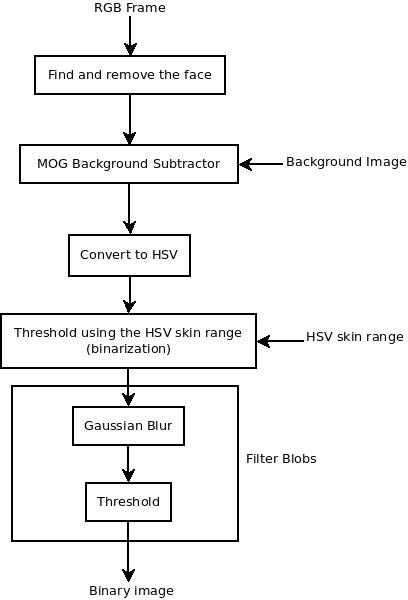
\includegraphics[scale=0.4]{../hand_filter.jpeg} 
 \end{center} 
 
As it can be seen in the diagram, the first thing done is to detect the face using the "Face Detection using Haar Cascades" already implemented in OpenCV. After this detection, a binary mask is made in which appear a black square over the face to hide it.

Next, a Mixture of Gaussians background subtractor is used to remove the background of the image and detect more easily the hand. From this step, another binary mask is created. 

Afterwards, the resulting image with the latter masks being applied is converted to the HSV color space and is thresholded using the appropriate HSV skin range.

Finally, in order to better the output binary image, a gaussian blur and a thresholding is applied to eliminate blobs and unite different regions of the hand. It was chosen this configuration because it was much faster and gave better results than making an opening to the image. 

 
\subsection{Hand Description}

The input of this section is the binary image that was the output of the previous one. This part of the software characterizes and extracts the hand's parameters. 
The flowchart is as follows: 

\begin{center}
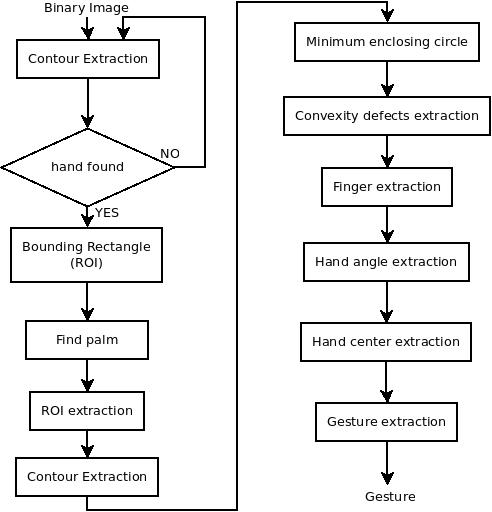
\includegraphics[scale=0.5]{../hand_description.jpeg} 
\end{center}

As it can be seen in the diagram, the first step is to extract the contours of the hand and decide from its size if it is a hand or only a blob remaining from the hand segmentation. 

If the size is appropriate, a bounding rectangle is found. Afterwards, the palm is extracted. In order to do that, a raw center of the palm and the radius of the inscribed circle is obtained from the points of the contour.

Then, the ROI (Region Of Interest), i.e. the rectangle that contains the maximum circle that represents the hand boundary.  

Afterwards, another contour extraction inside the extracted ROI is made in order to eliminate once more the smaller contours that may appear. 

Using the largest contour found in this last step, the minimum enclosing circle is obtained. This circle will be used as a hand's descriptor.

The following step is to compute the convexity defects, that will be used to extract the number of fingers present in the image. 
In order to assure that a certain part of the image is a finger, three conditions must be fulfilled: 
\begin{itemize}
\item The depth of the convexity defect must be in between the minimum inscribed radius and the maximum inscribed radius. 
\item The angle between the possible fingertips must be less than 90º. 
\item The fingertips must have a k-curvature inside a certain range.
\end{itemize}

In the next stage of the process, the angle of the hand is obtained measuring the angle of the minimum bounding box. A Kalman filter is placed in order to smooth the response of the system to sudden changes, that are assumed to be errors. 

Then, the hand center location is extracted using the center of the maximum inscribed circle and another Kalman filter to predict the position and eliminate the noise. 

Finally, the gesture made by the hand is extracted, taking as descriptors the number of fingers, the angle between fingers, and both the maximum and minimum inscribed circles. 

The output of this part of the software is a number that encodes the type of gesture made by the user.


\subsection{Gesture Recognition} 
This section of the software has as an input the output of the previous, again. Hence, it will implement a state machine that, depending on the input (the gesture) will execute one function or other. 

\begin{center}
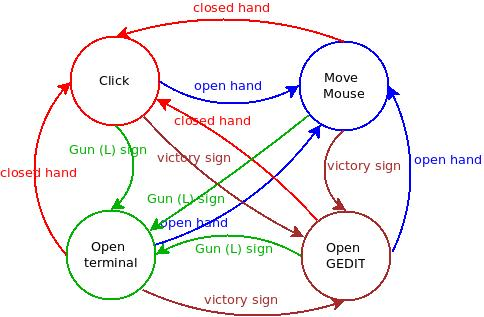
\includegraphics[scale=0.6]{../gesture_recognition.jpeg} 
\end{center}

The configuration of the actions to be made when an opened or closed palm appears is hardcoded in the program, since those values will not be changeables. In order to obtain the action for each of the two other gestures that may be customized, the software will read the configuration file, and execute the action specified in there. 

More information about the configuration file, the gestures and how to use the software in the following section "User Guide". 

\section{User Guide}
This code was developed using the following libraries: 
\begin{itemize}
\item OpenCV (v2.4.6.1).
\item X11 (linux native libraries that allows the control of the windows and mouse). 
\end{itemize}
The software was compiled using CMAKE (minimum version 2.8).
\\[0.5cm]
Therefore, those libraries are needed for the correct functioning of the software. 


\subsection{Compile the software [UBUNTU]}

In order to compile the code, there are various options. Here it will be explained how to compile using qt and terminal. 

To open the software as a Qt project, the only thing needed is to open the main CMakeLists.txt (gecko/CMakeLists.txt) with QtCreator. This will parse the whole project. 
Afterwards, press the "build" icon to build the project. 


The folder structure used is the typical of a CMake project. In order to compile using the terminal follow this steps: 
\begin{enumerate}
 \item Open a terminal in the build directory (gecko/build). 
 \item Enter the command "cmake ..". 
 \item Enter the command "make". 
\end{enumerate}

\subsection{Use the software}
In order to execute the software, press the convinient button of the QtCreator IDE or open a terminal in the bin directory (gecko/bin) and enter the command "./gecko.cpp". 

Once the code is compiled and started, a first window will appear with the information about the software. After pressing enter to continue, this menu will pop up: 
\begin{center}
\fbox{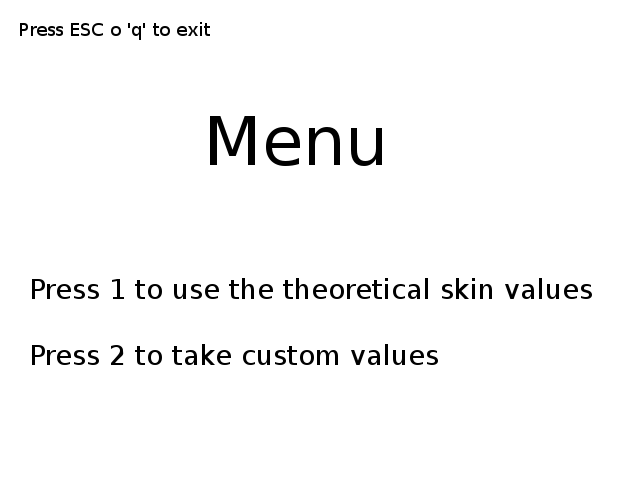
\includegraphics[scale=0.5]{../../img/menu.png} }
\end{center}

\vspace{1cm}
The first option will take the theoretical HSV skin values proposed in [1]. Afterwards, the application will allow us to adjust those HSV ranges to adecuate them to the room's conditions. 
Once all the adjustments are done, pressing ENTER will start the program. 

The second option will pop up a window with a green square in the middle. Place the hand so that the square is in the middle of your palm and press ENTER. The program will automatically calculate the HSV range of your skin. Afterwards you will be able once more to manually adjust those ranges. Pressing ENTER one last time will start the program. 
\\
 
The main program will track the hand and trace two circles, the first one around the palm and the second one surrounding the whole hand. The center of the palm is also shown, as well as the angle described by the hand. 

There are different functionalities implemented in this software. 
\begin{itemize}
\item Open hand(i.e. the program detects the five fingers): the mouse moves with the hand's movement.
\item Closed hand: click.
\item "Victory sign": the gedit text editor is opened.
\item "Gun or L sign": a terminal is opened. 
\end{itemize}

The two last functionalities may be changed using a configuration file named apps.config (gecko/data/apps.config). 
That configuration file contains the following:
\\[0.5cm]
\$gedit\$ 3 \\
\$gnome-terminal\$ 4
\\[0.5cm]
The three refers to the victory sign, and the 4 to the gun or L sign. To change the functionality the only thing needed is to change the programs written between the two dollar signs with the wanted one. 

\newpage
\section{Software Documentation}
\textbf{[PASTE DOXYGEN OUTPUT]}

\newpage
\section{Bibliography}

[1] H.-S. Yeo, B.-G. Lee, and H. Lim, “Hand tracking and gesture recognition system for human-computer interaction using low-cost hardware,” Multimed. Tools Appl., May 2013.
\\[1cm]
[2] A. Albiol, L. Torres, and E. J. Delp, “Optimum color spaces for skin detection,” no. 3, pp. 3–5.
\\[1cm]
[3] A. Argyros and M. Lourakis, “Tracking skin-colored objects in real-time,” Cut. Edge Robot., 2005.
\\[1cm]
[4] V. Vezhnevets, “A Survey on Pixel-Based Skin Color Detection Techniques,” 1994.



\end{document}